\documentclass[conference]{IEEEtran}
\usepackage[utf8]{inputenc}
\usepackage{cite}
\usepackage{graphicx}
\usepackage{amsmath,amssymb}
\usepackage{url}

\begin{document}

\title{Evaluating the Effectiveness and Sustainability of Modern Machine Learning Algorithms in Handling Attribute Noise}

\author{
\IEEEauthorblockN{Josef Almasri, Nawras Kanjo, Ahmad Haj Ahmad} \\
\IEEEauthorblockA{Assigned Supervisor: Vladislav Indykov}
}

\maketitle

\begin{abstract}
This thesis proposes an evaluation of how modern machine learning (ML) algorithms handle attribute noise errors in input features while considering both performance and sustainability. We will assess multiple supervised algorithms using traditional evaluation metrics, such as accuracy and F1 score, alongside sustainability indicators, including energy consumption and CO2 emissions.
    
The study aims to identify algorithms that maintain strong performance while minimizing environmental impact under varying levels of noise. By integrating sustainability into ML evaluation, this research seeks to provide practical insights for developing efficient, noise-resilient models for ML-enabled systems.
\end{abstract}


% ---------------------------
% I. INTRODUCTION
% ---------------------------
\section*{I. INTRODUCTION}
Artificial Intelligence (AI) enables systems to process data and make autonomous decisions. A key aspect of AI is Machine Learning (ML), which allows systems to learn from data, recognize patterns, automate tasks, and make predictions across various domains \cite{google_ai_ml}.
ML consists of models, each designed to handle specific types of data and tasks. The effectiveness of these models heavily depends on the quality and quantity of the data used for training.
However, training data often contains irrelevant, inconsistent, or false information, also called noise.
\newline
\newline
Noise is inevitable when collecting data from diverse sources, such as sensor readings (e.g., cars, medical equipment), online surveys, and websites. It can negatively affect machine learning performance and typically appears as attribute noise or class noise. Attribute noise refers to inconsistencies in input features (e.g., sensor errors, missing values), while class noise involves incorrect labels (e.g., misclassified images) \cite{dataheroes_noise}. 
\newline
\newline
Although both affect accuracy, class noise mainly misleads the model without significantly increasing computational cost. In contrast, attribute noise disrupts feature patterns, often requiring more training and computational resources \cite{wuzu}. This increased demand elevates energy consumption and CO2 emissions, aligning with Software Engineering (SE) concerns about sustainability, where non-functional requirements such as energy efficiency and environmental impact are critical to system design according to SWEBok v4 \cite[p. 69]{sweb}.
\newline
\newline
Our research focuses on attribute noise because it degrades model accuracy, efficiency, and sustainability. These inconsistencies can have significant real-world consequences, as seen in a well-known example from 2015, when Google Photos mistakenly labeled images of Black individuals as 'gorillas' \cite{guardian2015}. This accuracy error stemmed from imbalanced training data, where the system was exposed to more images of light-skinned individuals than darker-skinned ones. Such cases highlight the risks of attribute noise in real-world applications and reinforce the need for robust data quality measures in machine learning models.
\newline
\newline
Beyond degrading accuracy, noise also increases computational inefficiencies. Models exposed to noisy data often require longer training times, more iterations, and additional computing power to reach acceptable performance levels. This leads to higher energy consumption, amplifying the carbon footprint of machine learning applications \cite{sciencedirect}.
\newline
\newline
Given the escalating computational demands and environmental footprint of modern ML applications. According to Delanoe, Tchuente and Colin’s research \cite{DELAN}, training a large transformer model can emit an estimated 284,019 kg of CO2 (compared to 57,152 kg for a car’s lifetime or 16,400 kg per person annually). Evidence also suggests that machine learning could account for roughly 2\% of global carbon emissions by 2030 \cite{carbon_emissions}.
Thus, it is imperative to not only consider the traditional metrics, rather also account for sustainability. Traditional evaluation metrics include accuracy, precision, recall, and F1 score.
\newline 
\newline
This case study is critical because complex models often require substantial computational resources, and noise can increase resource utilization. By integrating both Traditional & Sustainability metrics, this research aims to offer a comprehensive understanding of the trade-offs involved when noisy data is present in ML training processes. This shift towards sustainability is becoming more evident as companies across various industries adopt eco-friendly practices, not only to protect the environment but also to reduce costs \cite{ey_ai_sustainability}. The increasing expenses of training machine learning (ML) models have made energy efficiency an important factor in AI development. Reports from Bain and EY emphasize the need to integrate sustainability into AI strategies, showing how energy-saving approaches can lower both costs and environmental impact \cite{bain_ai_sustainability}. 
\newline
\newline
The purpose of this study is to investigate the impact of different levels of attribute noise on selected ML models, by examining both traditional evaluation metrics and sustainability considerations. These metrics provide insights into how a model performs in the presence of noise. In parallel, sustainability, regarded as a Non-Functional Requirement (NFR), is assessed by measuring energy consumption and CO2e emissions during training.
\newline
\newline
The findings will provide insights into ML model selection to optimize energy use and reduce emissions. Consequently, this research will help machine learning engineers and researchers in AI-driven companies \& research institutions to assess which algorithms perform reliably on noisy, real-world data while promoting sustainable AI development.
\newline
\newline
The research will revise an assumption in the machine learning domain: that model selection is primarily based on traditional evaluation metrics such as accuracy and F1-score.  By demonstrating that environmental metrics (e.g., CO2 emissions) must be integrated alongside the traditional criteria, this study redefines what constitutes an effective algorithm. In addition, this research extends the knowledge because it is linking the chosen algorithms to CO2e emissions, thereby establishing a sustainability consideration for evaluating noise-resistant models. From an SE perspective, this aligns with long-term organizational demands, such as minimizing redundant computational work and optimizing resource allocation to reduce environmental and economic waste \cite[pp. 290-291]{sweb}.

% ---------------------------
% II. RELATED WORK
% ---------------------------
\section*{II. RELATED WORK}
Background: The world is becoming smarter everyday, a big part of this is the increasing dependency on machine learning across multiple fields. Allowing the rapid development of many ML models \cite{bain_ai_sustainability}. When training ML models, data imperfections like noise (e.g., errors, missing values, or inconsistencies) can disrupt learning and degrade predictions \cite{sciencedirect_noise}. Attribute noise, such as sensor errors or irrelevant feature variations, is particularly problematic as it distorts input patterns, increasing computational demands [12].\newline
\newline
Zhu and Wu \cite{wuzu} provided one of the foundational quantitative studies that clearly differentiated between class noise and attribute noise. Their systematic evaluation demonstrated that attribute noise defined as inconsistencies or errors in the input features can harm a model's performance more severely than class noise. Unlike class noise, which involves incorrect labels that might just mislead the model during training, attribute noise directly corrupts the data that the model learns from. Their study also showed that when the input features are noisy, the model struggles to identify the true patterns in the data, leading to poorer predictions and requiring more effort to learn correctly. This is why our research focuses on attribute noise: it poses a greater challenge by directly affecting the quality of the information fed into the model, making it critical to choose an ML model that best handles these errors while also being energy efficient.
\newline
\newline
This degradation that attribute noise causes, not only impairs predictive accuracy but also forces models to expend additional computational resources, thereby amplifying energy consumption and environmental impact \cite{wuzu}. Given these substantial repercussions, our research prioritizes attribute noise as a critical factor. By focusing on attribute noise, we aim to bridge the gap between traditional performance metrics and sustainability considerations, underscoring the need for robust, energy efficient machine learning practices in real world, noisy environments.

\newline
\newline
\newline
Building on our discussion of how attribute noise harms both model accuracy and energy efficiency, Chejara et al. \cite{chejara2024impact} provide concrete evidence from real-world settings that reinforces these concerns. Their study, conducted in authentic classroom settings using multimodal learning analytics, demonstrates that attribute noise significantly degrades model performance and reveals substantial differences in which algorithm is chosen under noisy conditions. For example, Chejara et al. \cite{chejara2024impact} report that when the quality of video or audio data is compromised such as when video frames become blurry or audio signals are distorted, the performance of the Support Vector Machine (SVM), a common machine learning model, drops notably. In contrast, another machine learning model, Random Forest, which combines the predictions of many decision trees, was observed to handle these imperfections much more gracefully, with only a marginal decline in performance. This happens because Random Forest builds multiple decision trees on different parts of the data; even if some trees are affected by noise, their errors are balanced out by the others. This clear disparity underscores the importance of selecting ML models addressing attribute noise directly. Our research aims to identify and promote ML models that can reliably handle real-world data imperfections while also minimizing environmental impact.
\newline
\newline
Abdulgalil and Abraham \cite{abduljalil} compared five machine learning algorithms which are Decision Tree (DT), Support Vector Machine (SVM), k-Nearest Neighbors (KNN), Naïve Bayes (NB), and Random Forest (RF) on a dataset of 768 instances containing feature-level noise (attribute noise), though the exact noise level was unspecified. Their findings revealed that SVM achieved the highest accuracy, F1-score, and precision but required significantly longer training times. Most strikingly, RF matched KNN’s accuracy, F1-score, and precision outcomes but was approximately 20 times slower to train, demonstrating that two algorithms with equivalent scores can have vastly different computational costs when it comes to energy consumption, lowering the sustainability of the algorithm. KNN itself trained the fastest while maintaining competitive results, whereas DT delivered moderate accuracy with reasonable training times, and NB provided good outcomes with minimal computational overhead. This 20x efficiency gap between RF and KNN, despite identical scores, epitomizes the trade-off between accuracy and computational efficiency under attribute noise, a key concern for sustainability, as prolonged training times directly increase energy consumption and environmental impact.
\newline
\newline 
Schooltink \cite{schooltink} compared the Support Vector Classifier(SVC) and Random Forest Classifier(RFC) to attribute noise by testing Gaussian and Mean-Based noise by looking at the mean accuracy and standard deviation. One dataset was used with around 88,500 instances. The Gaussian and Mean-Based noise are approaches to introduce synthetic noise into datasets. Under Gaussian noise, RFC usually has higher accuracy, but experiences a significant drop around 50\% noise, indicated by a larger standard deviation. The gap between the two algorithms' accuracy is notable when the noise is around 40\%. For the Mean based noise, both algorithms perform similarly until about 70\% of noise, after which SVC surpassed RFC. This means that SVC performs better in datasets that have a high level of attribute noise. 
\newline
\newline
Atla, Tada, Sheng, and Singireddy \cite{atla2011} conducted a study comparing how different machine learning algorithms react to attribute noise in datasets, with a primary focus on sensitivity comparisons across different noise levels. The metric that was used to compare the algorithms is accuracy. Naïve Bayes ' algorithm maintained roughly the same accuracy across different noise levels, while Decision Tree, Support Vector Machine, Logistic regression exhibited similar behaviour. Once the noise level exceeded 45\%, these three algorithms performed worse than Naïve Bayes. Making Naïve Bayes the most resistant to noise.
\newline
\newline
However, although each study addresses an important aspect of noise or sustainability, none provide a comprehensive evaluation that integrates traditional performance metrics with sustainability indicators (like energy consumption and CO2e emissions) across varying levels of attribute noise, while training the models. This gap underscores the significance and novelty of our proposed research. Our research aims to fill this gap by systematically assessing how different attribute noise levels affect both the effectiveness and the environmental impact of modern machine learning algorithms.


\section*{III. RESEARCH METHODOLOGY}
This study evaluates the effectiveness of modern ML algorithms in handling different levels of attribute noise while also measuring their environmental impact. Traditional metrics such as accuracy, precision, F1 score, and recall will assess how well algorithms perform under noisy conditions. To extend this evaluation, CO2 equivalent (CO2e) emissions will be measured during each model's training using the Code Carbon package. By analyzing both performance and environmental impact across varying noise levels, this study aims to provide valuable insights into the trade-offs between model effectiveness and sustainability for different algorithms under different levels of attribute noise.
\newline
\newline
Aim: To systematically evaluate how varying levels of attribute noise affect ML models' performance (via traditional metrics) and sustainability (via energy/CO2e measurements).
\newline

\subsection*{A. Research Questions and Hypotheses}
Main Research Question:
How do varying levels of attribute noise affect the performance and sustainability of supervised algorithms on boolean prediction values?
\newline
\newline
Sub-Questions:
\begin{itemize}
    \item 1. Do simpler models (e.g., Logistic Regression) degrade differently under noise compared to complex models?
    \item 2. How does attribute noise influence energy consumption and CO2e emissions during model training for boolean classification?
    \item 3. Which algorithm achieves the optimal trade-off between noise robustness and energy efficiency for boolean outcomes?
\end{itemize}
\newline
\newline
Hypotheses:
\begin{itemize}
    \item H1: Higher attribute noise levels will reduce traditional performance metrics non-linearly across models.
    \item H2: Energy consumption and CO2e emissions will increase with noise levels, but the rate will vary by each algorithm model.
    \item H3: Models with higher noise robustness (smaller performance degradation) will exhibit higher energy efficiency.
\end{itemize}
\newline
\newline
\subsection*{B. Research Methodology}
\textbf{Approach:} Comparative experimental study using supervised classification algorithms for target value of type boolean.
\newline
\subsubsection*{1) Data Collection}
\textbf{Datasets:} Use 2-3 boolean-labeled datasets from the Kaggle website \cite{kaggle}. Inject synthetic attribute noise (using Gaussian noise from 0\% to 100\% at 10\% increments) to simulate real-world data corruption.
\newline
\newline
\textbf{Algorithms:} 7 supervised classifiers for boolean prediction:
\begin{itemize}
    \item Logistic Regression (Baseline)
    \item Naive Bayes (Baseline)
    \item Random Forest (Ensemble)
    \item Gradient Boosting (Ensemble)
    \item Support Vector Machine (SVM) (Non-linear)
    \item k-nearest neighbors (KNN) (Non-linear)
    \item Decision Tree (Non-linear)
\end{itemize}

\begin{figure}[htbp]
    \centering
    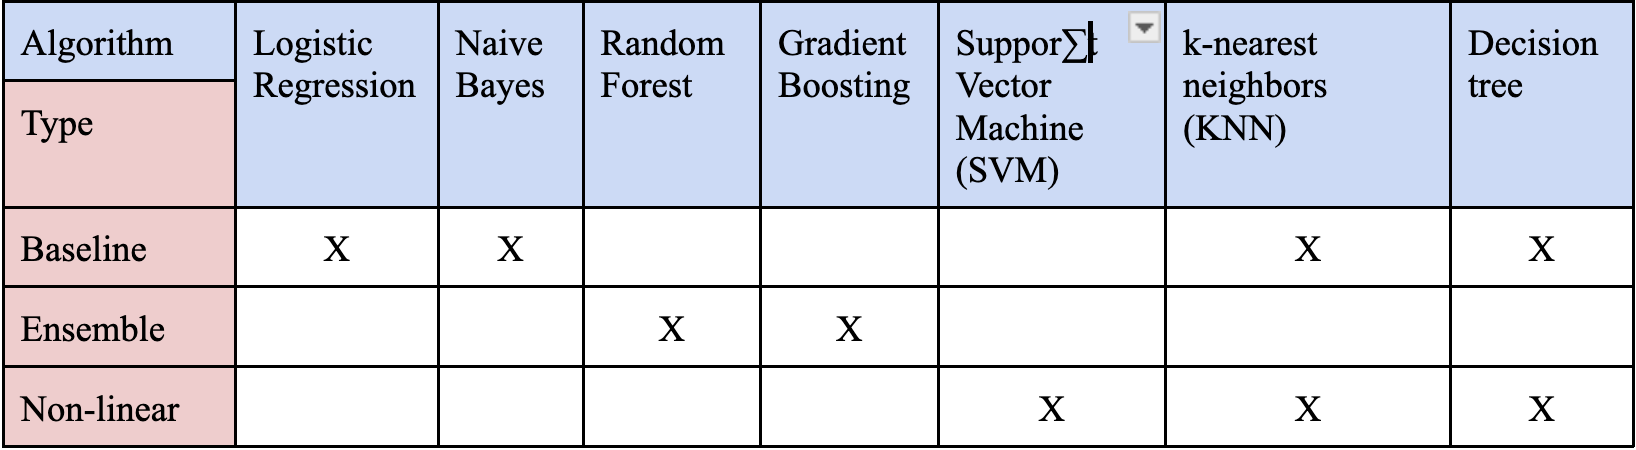
\includegraphics[width=\linewidth, keepaspectratio]{img.png} % Replace with your image file name -- MAKE SURE img.png EXISTS!
    \caption{Diagram of the algorithms used for boolean prediction.}
    \label{fig:algorithms}
  \end{figure}
Justification: These represent a gradient of complexity and noise-handling strategies.
\newline
\newline
\textbf{Metrics:}
\begin{itemize}
    \item Performance: Accuracy, precision, F1, and recall. These four metrics are chosen because they provide a balanced evaluation of classification performance, especially in cases with imbalanced data. While other metrics like AUC-ROC or MCC exist, these four are widely used, easy to interpret, and effectively capture both overall correctness (accuracy) and the trade-off between false positives and false negatives (precision, recall, and F1 score).

    \item Sustainability: Energy (kWh), CO2e (kg) per training cycle (measured via tools).

\end{itemize}

\textbf{Controls:}
\begin{itemize}
    \item Fix training parameters (epochs, batch size) across models.

    \item Use identical hardware (CPU/GPU) for all experiments (Same Computer).
\end{itemize}




\subsubsection*{2) Data Analysis}
\textbf{Performance Analysis:}
\begin{itemize}
    \item Compare accuracy, F1-score, and recall degradation curves across noise levels.
\end{itemize}

\textbf{Sustainability Analysis:}
\begin{itemize}
    \item Calculate energy per accuracy point to quantify efficiency.
    \item Rank models by CO2e emissions at equivalent noise levels.
\end{itemize}

\textbf{Trade-off Visualization:}
\begin{itemize}
    \item Visualization charts to compare algorithms across noise, accuracy, and energy use (Python).
    \item Scatter plots showing Energy per Accuracy (EPA) vs. noise tolerance.
\end{itemize}

\subsection*{C. Validity Threats}
\textbf{Internal Validity:}
\begin{itemize}
    \item Threat: Hyperparameter tuning could confound energy/performance results.
    \item Mitigation: Use default or standardized hyperparameters from previous literature for fairness.
\end{itemize}

\textbf{External Validity:}
\begin{itemize}
    \item Threat: Results may not generalize beyond boolean tasks or synthetic noise.
    \item Mitigation: Validate findings on 2-3 boolean datasets (e.g., medical, financial).
\end{itemize}

\textbf{Construct Validity:}
\begin{itemize}
    \item Threat: Energy measurement tools may not account for hardware-specific fluctuations.
    \item Mitigation: Replicate experiments on multiple hardware setups (CPU vs. GPU) and then take the average results of the traditional metrics and sustainability outcome.
\end{itemize}

% ---------------------------
% REFERENCES
% ---------------------------
\bibliographystyle{IEEEtran}
\bibliography{references}

\end{document}